%%
%% Author: dariochinelli
%% 2021-03-18
%%

\section{Modelli atomici}


%% ----------------------------------------------------------------------------------------------------------------------------------------
\subsection{Atomo di Thomson}
Nel 1904 Thomson propose il modello atomico detto a \textit{panettone}, per il quale l'atomo è costituito da una distribuzione di carica positiva diffusa dove all'interno si trovano inserite le cariche negative.
Tale atomo complessivamente neutro, risulterebbe sostanzialmente pieno e gli elettroni sarebbero fissi nelle posizioni di equilibrio e regolari. 
All'epoca si considerava il \textbf{raggio atomico} $r \sim \SI{1}{\AA}$, stimato considerando la densità di un solido, il suo peso atomico ed il numero di Avogadro.
Nello stato di più bassa energia gli elettroni sono fissi in posizioni di equilibrio, mentre per atomi eccitati (a cui viene fornita energia ad esempio riscaldando il materiale) si ha una vibrazione intorno alla posizione di equilibrio emettendo onde elettromagnetiche.
Questo modello ha molti problemi, tra cui non riuscire a spiegare completamente gli spettri atomici e l'esperimento di scattering delle particelle alfa.
Fu Rutherford a smentire il modello a panettone.


\paragraph{Esperimento di Rutherford (1911): scattering di particelle $\alpha$}
Venne fatto incidere un fascio di particelle $\alpha$, un atomo di Elio doppiamente ionizzato quindi di carica positiva, emesso da una sorgente radioattiva, contro una sottile lamina d'oro, il cui spessore era di poche migliaia di atomi.
\begin{figure}[h]
\centering
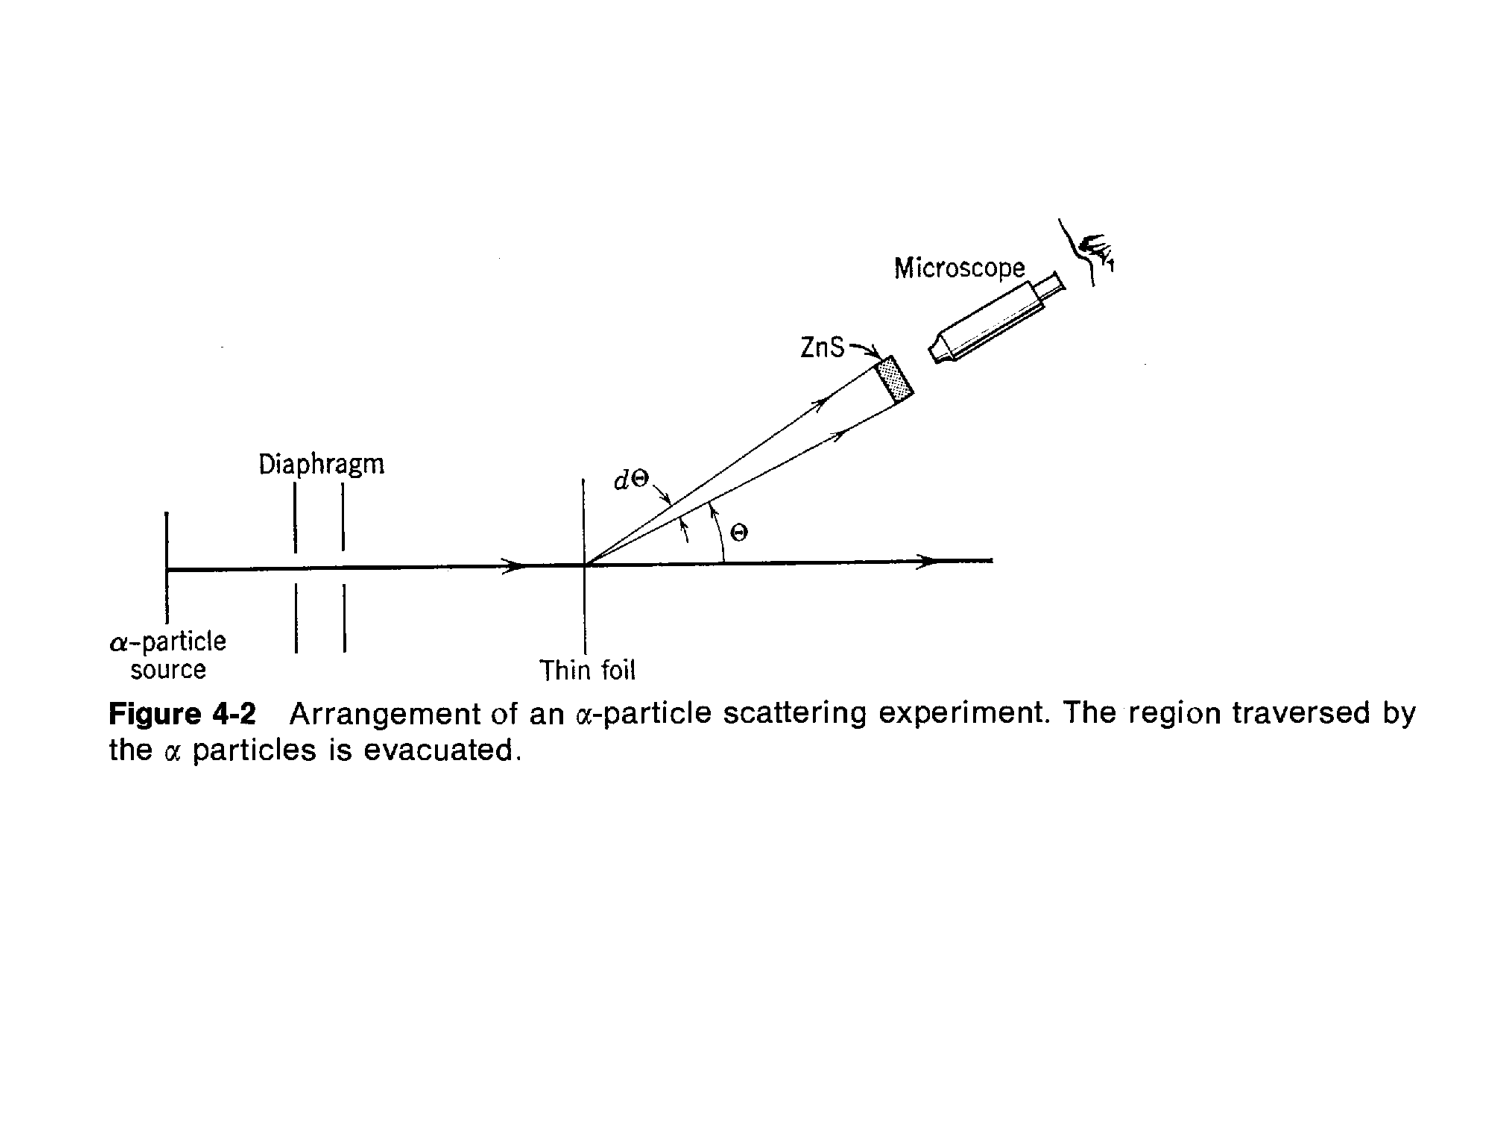
\includegraphics[scale=0.5]{/ruth_alpha}
\caption{Schema esperimento di Rutherford}
\end{figure}
Venne posizionato uno schermo fluorescente (ZnS) tutto intorno alla lamina d'oro, in modo da evidenziare il passaggio di ogni particella alfa.
In questo modo fu possibile ricostruire la traiettoria percorsa dalle particelle dopo la diffusione con la lamina.
Secondo il modello Thomson le particelle avrebbero dovuto attraversare il foglio d'oro ed uscire con una traiettoria variata di al più di pochi gradi, quindi poco diffuse.
\begin{figure}[h]
\centering
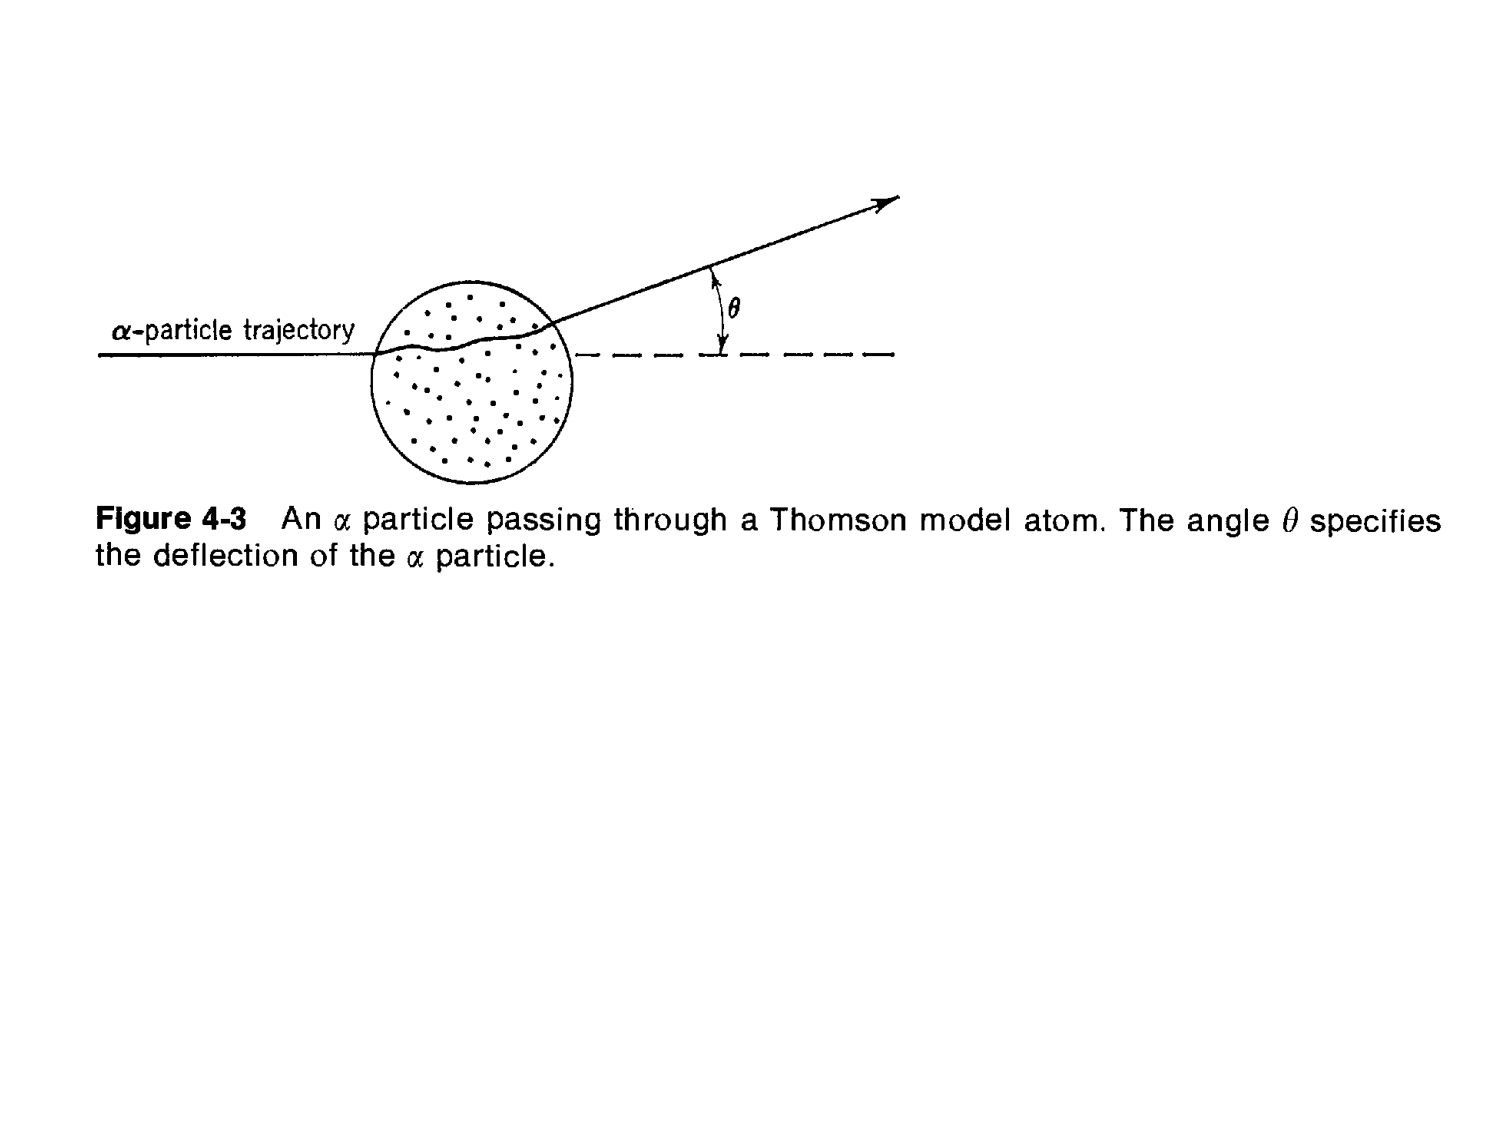
\includegraphics[scale=0.5]{/thomson_alpha}
\caption{Se vale il modello di Thomson}
\end{figure}
Misurando la diffusione delle particelle si poterono ricavare informazioni sulla distribuzione della carica elettrica all'interno dell'atomo.

Sia $N$ il numero di atomi che deflettono una particella alfa nel suo passaggio attraverso la lamina.
La formula seguente unisce l'angolo di scattering $\Theta$, ovvero l'angolo di deflessione totale della particella nel passaggio dell'intera lamina e l'angolo della deflessione $\theta$ causata da un atomo solo.
\begin{equation}
\begin{split}
& \Bigl(  \overline{ \Theta^2 }  \Bigr)^{ \frac{ 1}{2 } } = \sqrt{N} \Bigl(  \overline{ \theta^2 }  \Bigr)^{ \frac{ 1}{2 } } \\ 
& N(\Theta)d\Theta = \frac{2 I \Theta}{\overline{\Theta^2}} e^{-{\Theta^2}/{\overline{\Theta^2}}} d\Theta
\end{split}
\end{equation}
$N(\Theta)d\Theta$ esprime il numero di particelle diffuse in un angolo $d\Theta$. 
In cui $I$ rappresenta il numero di particelle $\alpha$ che attraversano la lamina.
L'esponenziale descrive come il numero di particelle diffuse diminuisca drasticamente all'aumentare dell'angolo di scattering.

\begin{figure}[h]
\centering
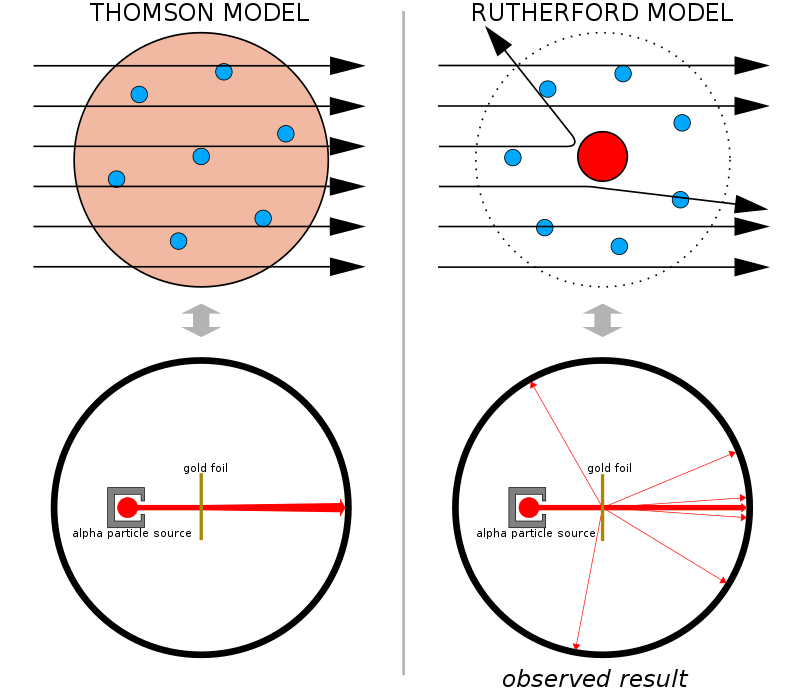
\includegraphics[scale=0.44]{/Geiger_Marsden_experiment_expectation_and_result}
\caption{ Confronto tra i due modelli }
\end{figure}

Questa formula si ottiene trascurando le interazioni Coulombiane tra le particelle $\alpha$ e gli elettroni (la cui massa è assai piccola) e si conta solo la deflessione dovuta alla parte positiva dell'atomo.
Secondo Thomson, se la carica positiva fosse stata distribuita in modo continuo, non sarebbe possibile avere $\theta$ grandi poiché deve essere $\theta \le \SI{e-4}{rad}$.

A questo proposito si consideri l'esperimento di Geiger e Marsden (1909).
Sperimentalmente venne accertato che alcune particelle, 1 su 8000, venivano diffuse ad angoli maggiori di $\frac{ \pi}{2 }$, evento completamente imprevisto da Thomson, ma in accordo con Rutherford.

\paragraph{Esempio} 
dato lo spessore della lamina d'oro pari a \SI{e-6}{m} e sia l'angolo medio di scattering pari a $(\overline{\Theta^2})^{1/2} = 2\cdot 10^{-2} RAD$ , si calcoli $(\overline{\theta^2})^{1/2}$

$$ N = \frac{\SI{e-6}{m}}{\SI{e-10}{m}} = 10^{-4} $$
$$(\overline{\theta^2})^{1/2} = \frac{(\overline{\Theta^2})^{1/2}}{\sqrt{N}} = \frac{2\cdot 10^{-2}}{10^{2}} = 2 \cdot 10^{-4} RAD $$


%% ----------------------------------------------------------------------------------------------------------------------------------------
\subsection{Modello di Rutherford}
Tutta la carica positiva è concentrata nel \textit{nucleo} di raggio $r = \SI{e-14}{m}$.
In questo modello una particella alfa che passi molto vicino ad esso può essere scatterata da una forza repulsiva ed essere deviata di angoli molto ampi.
Rutherford calcolò la distribuzione angolare assumendo che lo scattering fosse solo tra la particella $\alpha$ ed il nucleo, ignorando l'interazione coulombiana con gli elettroni: gli elettroni avendo massa molto più piccola producono deflessioni a piccoli angoli.
Considera quindi solo la forza coulombiana tra la particella $\alpha$ e il nucleo, considerandolo fisso nello spazio durante l'urto ed imponendo che la particella non possa entrare nel nucleo: equivale a considerare i due oggetti come puntiformi.
\begin{figure}[h]
\centering
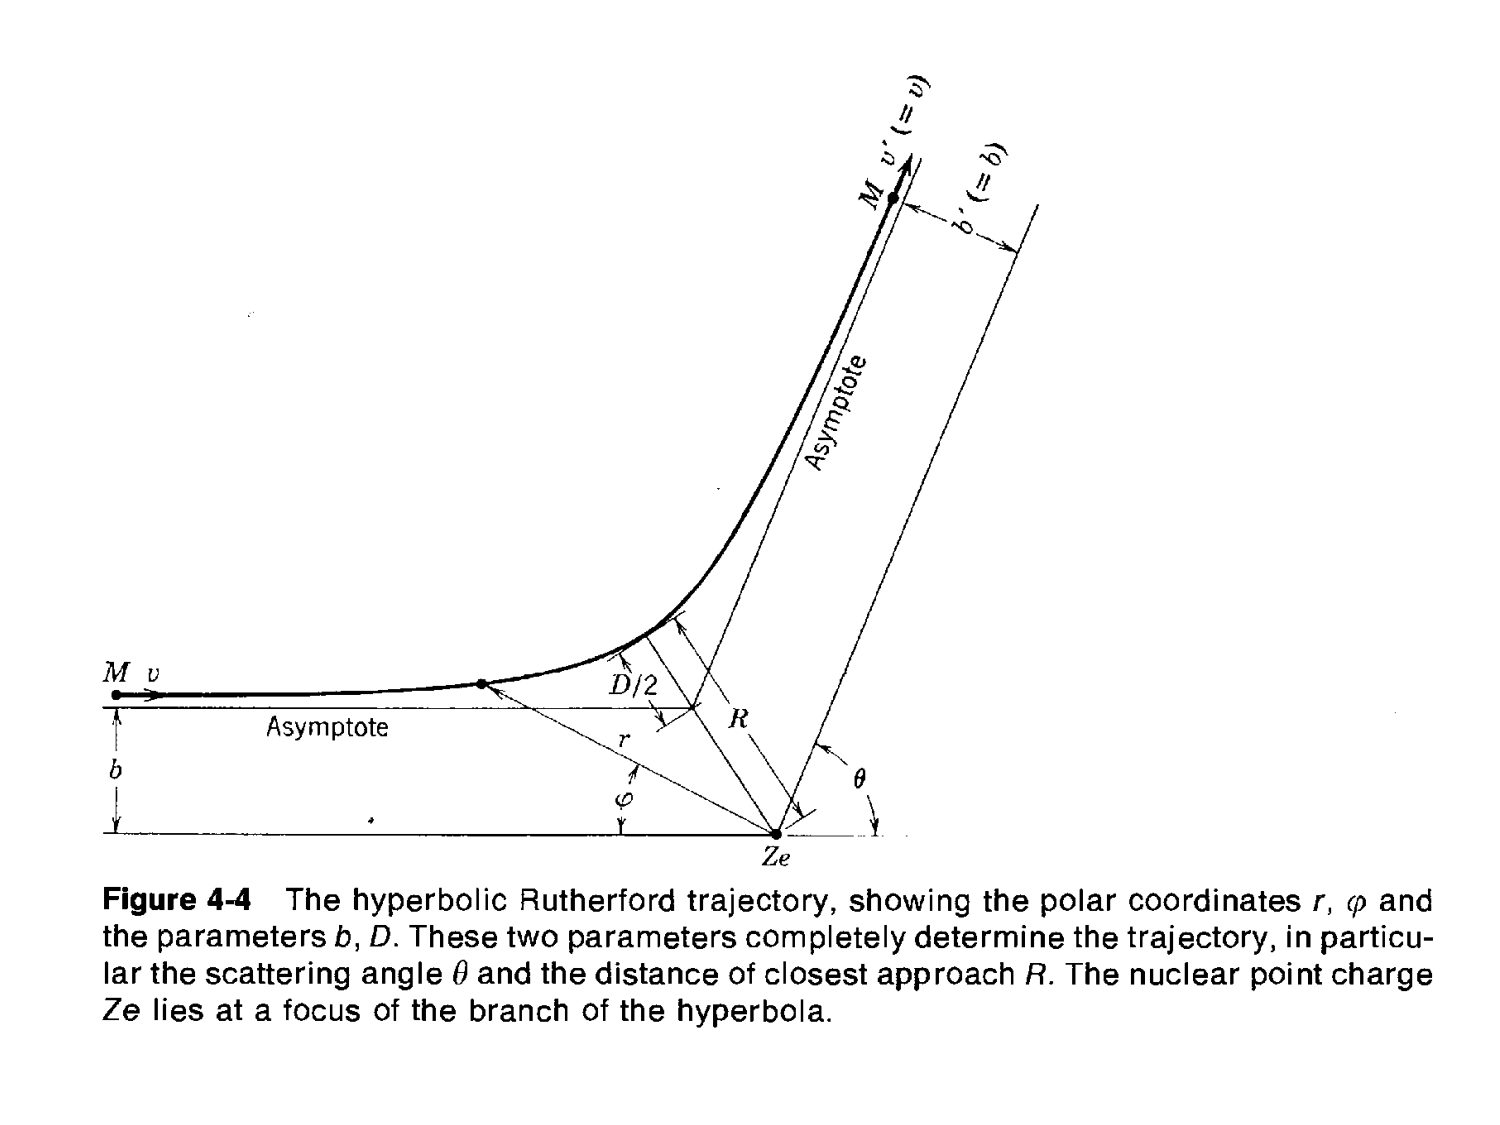
\includegraphics[scale=0.5]{/iperbole}
\caption{Iperbole di deflessione della particella da parte del nucleo}
\end{figure}
In cui notiamo che i moduli delle velocità iniziale e finale della particella $\alpha$ siano uguali.
L'angolo $\varphi$ descrive la posizione in coordinate polari.
L'angolo $\theta$ è l'angolo di deflessione.
$D$ è una costante che corrisponde alla distanza di avvicinamento minima in una collisione frontale, ovvero dove l'energia potenziale coulombiana è uguale all'energia cinetica della particella (vedi eq \ref{v_k}).
\begin{equation}
F = \frac{z Z e^2}{4\pi \epsilon_0 r^2}
\end{equation}
da cui si ottiene
\begin{equation}
\frac{1}{r} = \frac{\sin \phi}{b} + \frac{D}{2 b^2} ( \cos \phi - 1 )
\end{equation}
dove $b$ è il parametro di impatto
\begin{equation}
\begin{split}
& D = \frac{1}{4\pi \epsilon_0} \frac{z Z e^2}{M r^2/2} \\
& \frac{1}{4\pi \epsilon_0} \frac{z Z e^2}{D} = \frac{ 1}{2 } M v^2
\end{split}
\label{v_k}
\end{equation}

L'angolo $\theta$ di scattering segue il valore di $\varphi$ quando $r \rightarrow \infty $ e ponendo $\theta = r - \varphi $, da cui:
\begin{equation}
\begin{split}
& \lim_{x\to\infty} \bigg\{  \frac{1}{r} = \frac{\sin(r - \theta)}{b} + \frac{D}{2 b^2} [ \cos (r - \theta) - 1 ] \bigg\} = 0 \\
& \sin \theta = \frac{D}{2 b} (\cos \theta + 1) \\
& \frac{2 b }{D} = \frac{\cos \theta + 1}{\sin \theta} = \frac{ [\cos^2 (\theta /2) - \sin^2 (\theta /2) ] + [ \sin^2(\theta /2) + \cos^2(\theta /2) ] }{  2 \sin(\theta /2) \cos(\theta /2)  }
\end{split}
\end{equation}

\begin{equation}
\cot(\theta /2) = \frac{2 b}{D}
\label{angolo_di_scattering}
\end{equation}
Da cui si deduce che se nello scattering di una particella alfa con un singolo nucleo è nel range da $b$ a $b + db$ allora l'angolo di scattering sarà nel range $[\theta, \theta + d\theta]$.
Un'altra formula importante è quella della distanza di avvicinamento minima è data da
\begin{equation}
\begin{split}
& R = \frac{ D}{2 } \Bigl[ 1 + \frac{ 1}{\sin\Bigl(  \frac{\theta}{2 }  \Bigr) } \Bigr] \\
& \mbox{t.c. se} \quad \theta \to \pi \quad (b=0) \quad \Rightarrow \quad R \to D \\
& \mbox{t.c. se} \quad \theta \to 0 \quad (b=\infty) \quad \Rightarrow \quad R \to \infty
\end{split}
\end{equation}

Ebbene il problema di calcolare il numero $ N(\Theta) d\Theta$ delle particelle alfa scatterate nel range angolare $[\Theta, \Theta +d\Theta]$ nell'attraversare la lamina è equivalente al problema di calcolare il numero di quelle incidenti, con un parametro d'impatto nel range $[b, b +db]$.
Da cui si ottiene la formula di Rutherford:
\begin{equation}
N(\Theta)d\Theta = \biggl( \frac{1}{4\pi \epsilon_0} \biggr) ^2  \biggl( \frac{z Z e^2}{2 M v^2} \biggr)^2  \frac{ 2 \pi I \rho t  \sin\Theta d\Theta }{ \sin^4(\Theta/2) }
\label{scattering_rutherford}
\end{equation}
Dove $I$ è il numero di particelle alfa che incidono sulla lamina di spessore $t$.
Anche questa formula prevede una decrescita del numero di particelle all'aumentare dell'angolo, ma in modo più lieve rispetto al modello precedente di Thomson.
Da questo modello si vede che è possibile un \textit{back scattering} anche nell'interazione con un solo nucleo.

Si vede che, se comparato al modello di Thomson, sebbene in entrambi i casi il fattore angolare decresce rapidamente all'aumentare di $\Theta$, tale decrescenza è decisamente più precisa per le predizioni di Rutherford.
La formula di scattering di quest'ultimo è tale che il numero di $dN$ di particelle $\alpha$ scatterate in un angolo solido $d \Omega$ ad un angolo di scattering sia:
\begin{equation}
dN =  \frac{ d\sigma }{d\Omega} I n d\Omega
\end{equation}
Dove $I$ è il numero di particelle alfa incidenti sulla lamina sottile contenente $n$ nuclei per centimetro quadrato.
La definizione è analoga alla definizione di \textit{cross section}
\begin{equation}
N = \sigma I n
\end{equation}
e considerando che $d\Omega = 2\pi\sin\Theta d\Theta$, si riscrive la formula di scattering come differenziale
\begin{equation}
\begin{split}
& dN =  \biggl( \frac{1}{4\pi \epsilon_0} \biggr) ^2  \biggl( \frac{z Z e^2}{2 M v^2} \biggr)^2  \frac{ I e t 2 \pi \sin\Theta d\Theta }{ \sin^4(\Theta/2) } \\
& \frac{ds}{d\Omega} = \biggl( \frac{1}{4 \pi \epsilon_0} \biggr)^2  \biggl( \frac{z Z e^2}{2 M v^2} \biggr)^2  \frac{ 1 }{ \sin^4(\Theta/2) }
\end{split}
\end{equation}




\paragraph{Problemi nel modello di Rutherford}
Il modello di Rutherford non era però in grado di spiegare alcuni fenomeni.
\begin{enumerate}

\item Alte energie di impatto \\
Degli esperimenti in cui si fa variare l'energia delle particelle incidenti evidenziarono che oltre un certo valore di energia pari a $\SI{27.5}{MeV}$ il modello di Rutherford è completamente in disaccordo con i dati sperimentali.
\begin{figure}[h]
\centering
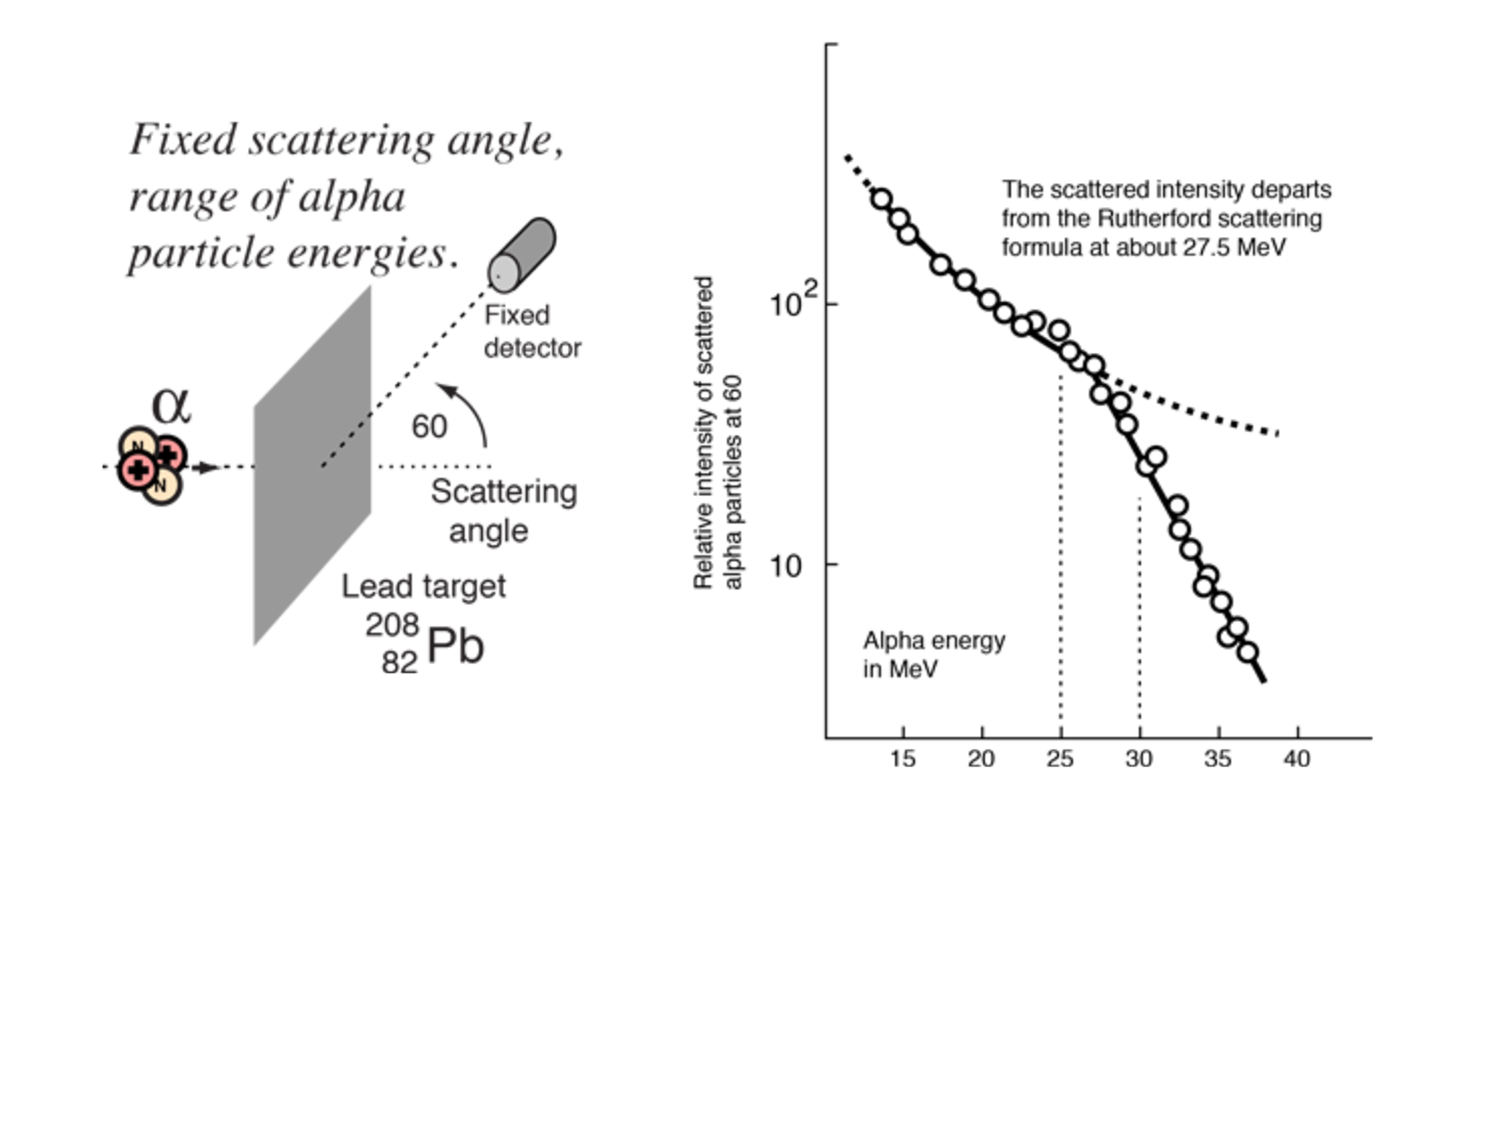
\includegraphics[scale=0.5]{/errore_ruth}
\caption{Il grafico mostra che oltre una certa energia il modello di Rutherford non funziona più e che subentrano altre interazioni}
\end{figure}

\item Stabilità dell'atomo \\
Se immaginiamo che gli elettroni siano fermi intorno al nucleo, questi dovrebbero cadere sul nucleo sotto l'azione coulombiana, quindi non possono essere fermi ed in tal caso l'intero atomo avrebbe le dimensioni del nucleo, e non è così.
Allora si può pensare agli elettroni orbitanti intorno al nucleo, ma siccome sono cariche accelerate dovrebbero emettere energia sotto forma di onde elettromagnetiche e perderebbero energia al punto da cadere sul nucleo: di nuovo l'atomo dovrebbe coincidere con le dimensioni del nucleo.

\item Spettro atomico discreto \\
Gli elettroni dovrebbero irradiare energia sotto forma di onde elettromagnetiche con uno spetto continuo della radiazione emessa, ma ciò che si osserva negli esperimenti che sono spettri atomici discreti.
\end{enumerate}

\subsection{Spettri atomici} 
Quando si parla di spettro atomico si fa riferimento all'emissione elettromagnetica discreta di un gas monoatomico.
Gli spetti atomici possono essere osservati utilizzando una scarica elettrica passante attraverso una regione contenete il gas.
A causa della scarica, e della collisione tra atomi, gli elettroni di alcuni degli atomi si pongono in uno stato energetico in cui la loro energia totale è maggiore di quella di un atomo non eccitato.
Tornando poi ad uno stato energetico inferiore, l'eccesso di energia si manifesta attraverso l'emissione di radiazione elettromagnetica: un fotone.
Essa viene poi collimata da una fessura (diaframma) e fatta passare attraverso un prisma, è possibile allora osservare sulla lastra fotografica uno spettro discreto.
Ogni tipo di atomo ha un suo spettro caratteristico, quindi lunghezze d'onda ben precise.
\begin{figure}[h]
\centering
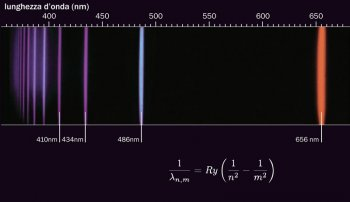
\includegraphics[scale=1]{/INFN_Asimmetrie22_pag8_img1}
\caption{ Le righe spettrali emesse nel visibile dall’atomo di idrogeno. Le prime quattro da destra furono osservate inizialmente da Ångström. I valori osservati vengono riprodotti dalla formula di Rydberg-Balmer fissando Ry=10.9721 cm-1 e n=2, per m=3,4,5,6. }
\end{figure}
Nel 1885 \textit{Johann J. Balmer} osservò che alcune righe dello spettro di emissione dell'idrogeno possono essere calcolate utilizzando la \underline{formula di Balmer}:
\begin{equation}
\lambda = 3646 \frac{n^2}{n^2 - 4} \quad \mbox{ (in $\AA$}
\end{equation}
Righe di emissione dell'idrogeno:
\begin{itemize}
\item $H_{\alpha}$ $n=3$ $\rightarrow$ red $\lambda = \SI{6562.8}{\AA}$
\item $H_{\beta}$ $n=4$ $\rightarrow$ blue $\lambda = \SI{4861.3}{\AA}$
\item $H_{\gamma}$ $n=5$ $\rightarrow$ violet $\lambda = \SI{4340.5}{\AA}$
\end{itemize}
Balmer suppose che tale formula fosse, in realtà, un caso particolare di una legge più generale.
Infatti tale formula venne trovata da \textit{Johannes Rydberg} e \textit{Walther Ritz}, sempre relativa all'idrogeno
\begin{equation}
\begin{split}
& k = \frac{1}{\lambda} = R_H \biggl( \frac{1}{n_1^2} - \frac{1}{n_2^2}  \biggr) \\
& \mbox{con } n_{1} \mbox{, } n_{2} \in \mathbb{N} > 0 : n_{1} < n_{2} \\
& R_H = \SI{10.9721}{cm^{-1}} \quad R \mbox{ dell'idrogeno}
\end{split}
\end{equation}
Chiamata \underline{formula di Ridberg Ritz} (1908)
\begin{equation}
k = \frac{1}{\lambda} = R \biggl[ \frac{1}{(m-a)^2} - \frac{1}{(n-b)^2}  \biggr]
\end{equation}
Dove $a, b$ sono fissi per una data serie, $m$ è un intero fisso e $n$ è un intero variabile.
Si scoprirono altre serie di linee come mostrato in figura \ref{serie_linee} e che per tutti gli elementi alcalini le formule associate hanno tutte la stessa struttura.
\begin{figure}[h]
\centering
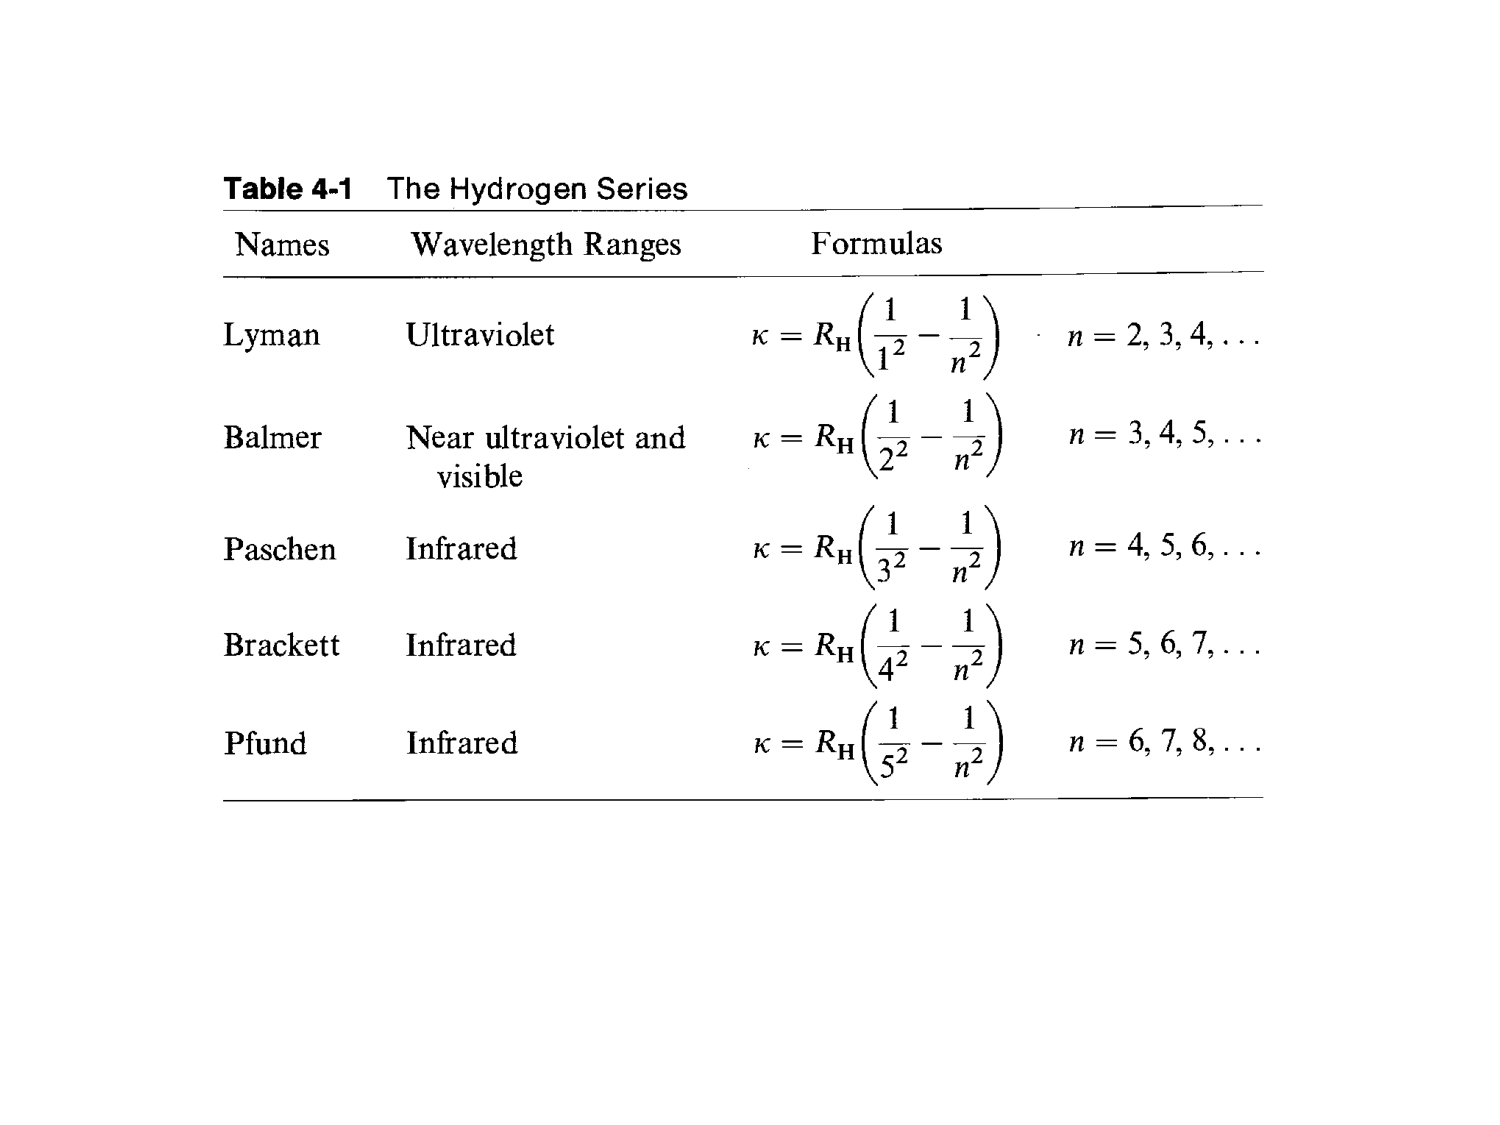
\includegraphics[scale=0.6]{/serie_linee_idrogeno}
\caption{CAPTION}
\label{serie_linee}
\end{figure}
Questo fatto che lo spettro fosse discreto e non continuo era inspiegabile con i modelli atomici di Thomson e Rutherford. 
Occorre sapere che per ogni riga dello spettro di emissione ce n'è una nello spettro di assorbimento.
\begin{figure}[h]
\centering
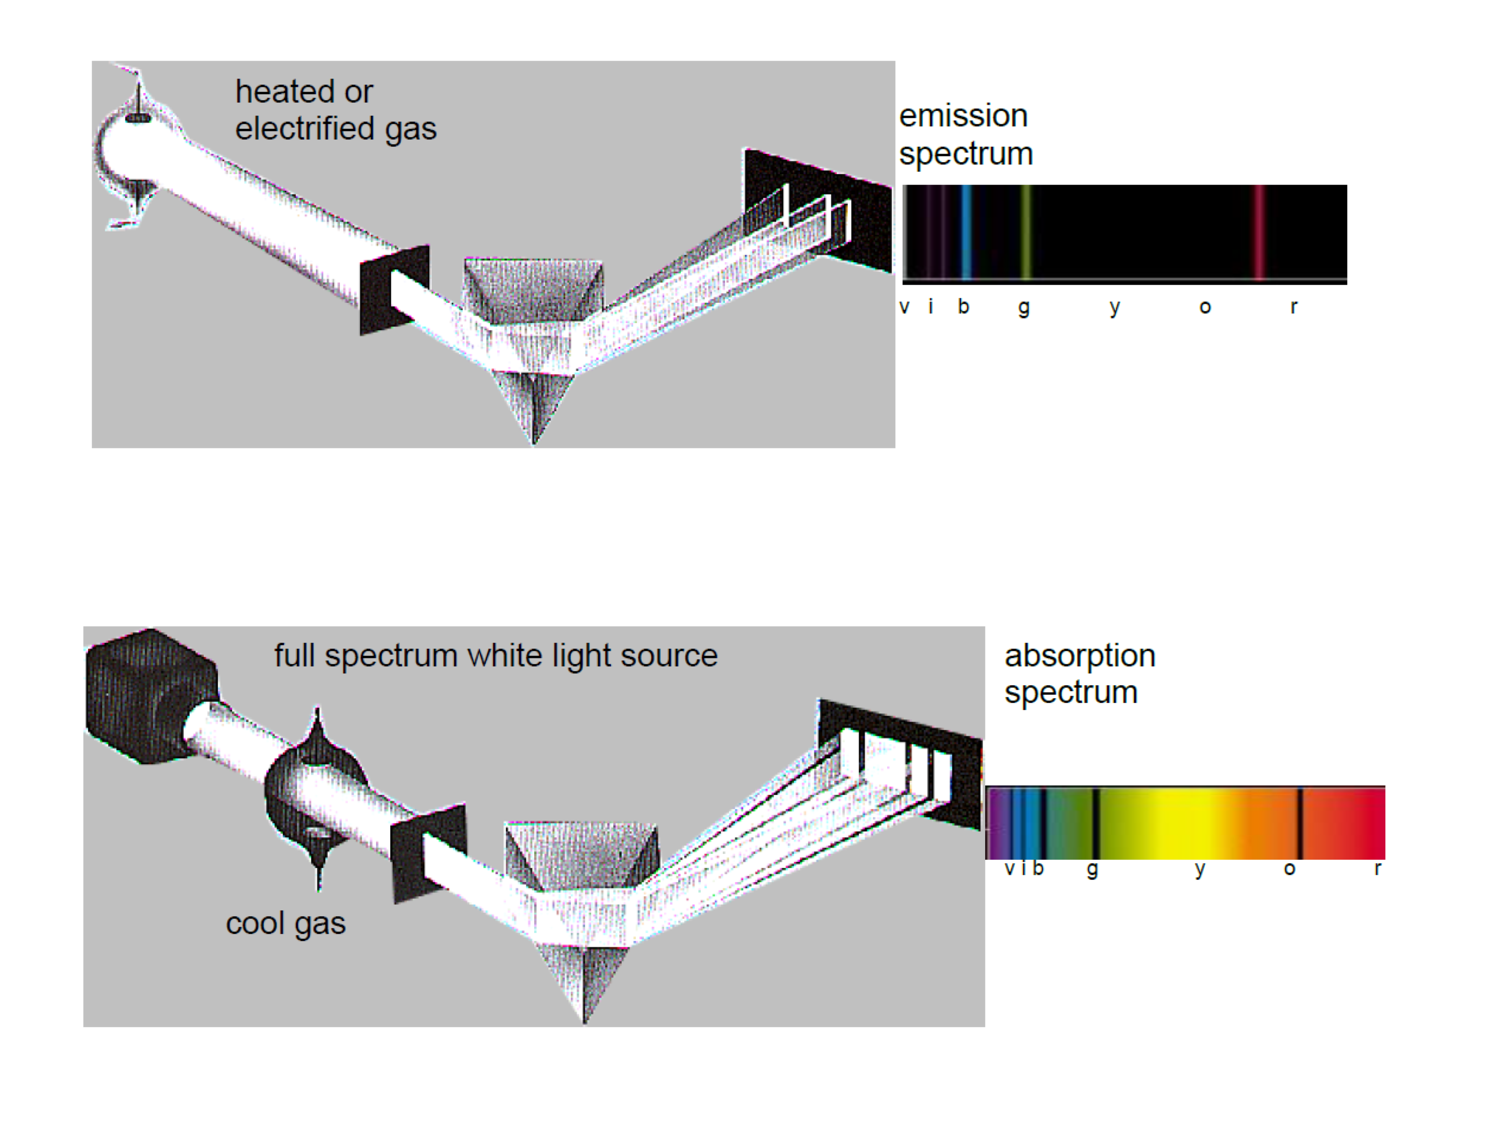
\includegraphics[scale=0.5]{/linee_assorbimento_emissione}
\caption{Oltre allo spetto di emissione si studia anche lo spettro di assorbimento}
\end{figure}



%% ----------------------------------------------------------------------------------------------------------------------------------------
\subsection{Modello atomico di Bohr}








%% ----------------------------------------------------------------------------------------------------------------------------------------
\subsection{Modello di Wilson-Sommerfeld}








